\section{Formal Analysis using Alloy}

\subsection{Queue Modeling}
Queue management is one of the most critical aspects of the application.
We implemented the concept of queue as a set of ordered Tickets.
We made the assumption that each customer will stay at least one unit of time inside of the store to be able to model it through Alloy Int variables. 
To create a fully populated world we used one fact to have all the slot assigned to at least one ticket. 
We checked that no slot inside of the store is assigned to multiple people at the same time, by respecting the registered entrance and exit time. 

\lstinputlisting[language=C]{alloy/queue.als}
\begin{figure}[H]
    \centering
    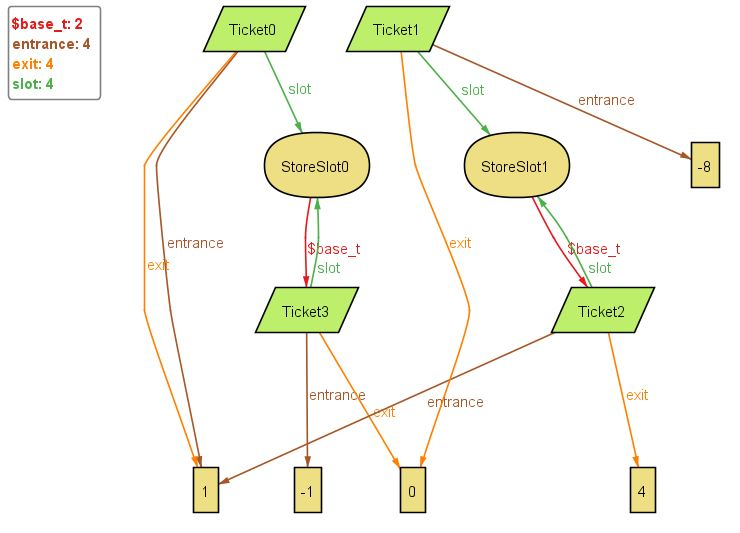
\includegraphics[width=1\textwidth]{alloy/Line_Alloy.JPG}
    %\caption{Enter Store from Queue Sequence Diagram}
\end{figure}

\subsection{Reservation Modeling}
\lstinputlisting[language=C]{alloy/reservations.als}
\begin{figure}[H]
    \centering
    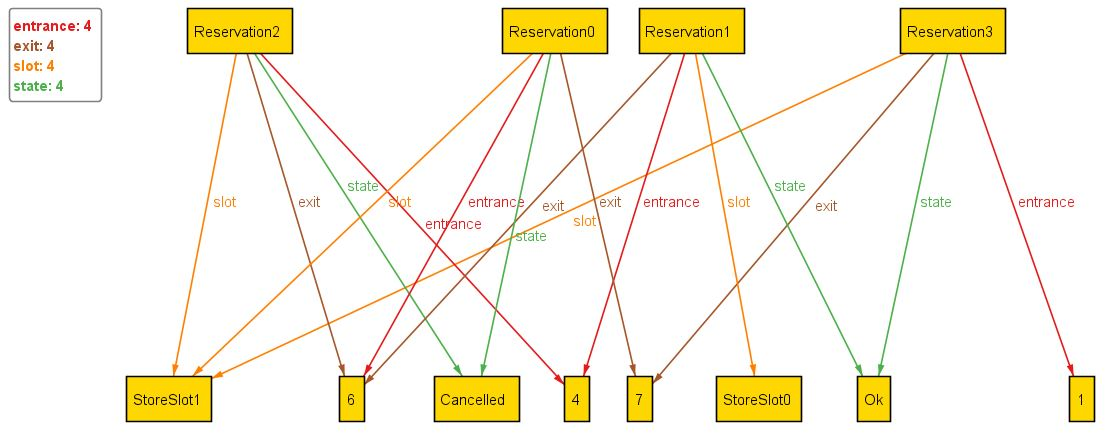
\includegraphics[width=1\textwidth]{alloy/Reservation_Alloy.JPG}
    %\caption{Enter Store from Queue Sequence Diagram}
\end{figure}
